\subsection{Design av kolonnefamiliedatabasen}
Her brukte vi datasettet "World University Rankings" med Times Higher Education World University Ranking metodikken.

\subsubsection{Begrunnelse bak valgene rundt kolonnefamilie- og grafdatabase}
Begge har raske queries. Vi vil gjerne vite om alle skoler basert på forskjellige faktorer, og vi ønsker å gjøre det  mange ganger med forskjellige variabler. I tillegg hjelper det spesielt at en kan selv velge grad av konsistens ved en read/write. En kan altså her velge selv hvor mange av nodene en write skal kjøres på, og replikering av nodene kan gjøres etter behov. Skalerbarheten er massiv, og når det kommer hyppig med queries, vil det ikke nesten ikke merkes.

\subsubsection{Hvorfor kolonnedatabase?}
Grunnen til at vi har valgt kolonnedatabase for dette datasettet er blant annet fordi 
kolonnedatabaser tilbyr svært rask lesing og og skrive-spørringer. Dette er nyttig, siden vi bruker et 
stort datasett med mange rader. I tillegg er kolonnefamiliedatabaser mer egnet for AP-systemer, 
som vil si at den prioriterer tilgjengelighet over konsistens. Dataen i dette datasettet oppdateres ikke 
ofte (maksimalt en gang i året), og ved hjelp av timestamps for hver verdi vil ikke konsistensen være 
et stort bekymring

\subsubsection{Aggregeringer}
% Aggregering 1 %
\textbf{Rådata}\\
Dette dataobjektet representerer rådata brukes til å oppdatere dataen i databasen. Dette objektet opprettes når ny data blir lest inn, eller når bruker legger inn selv.

\FigureCounter
\begin{figure}[H]
  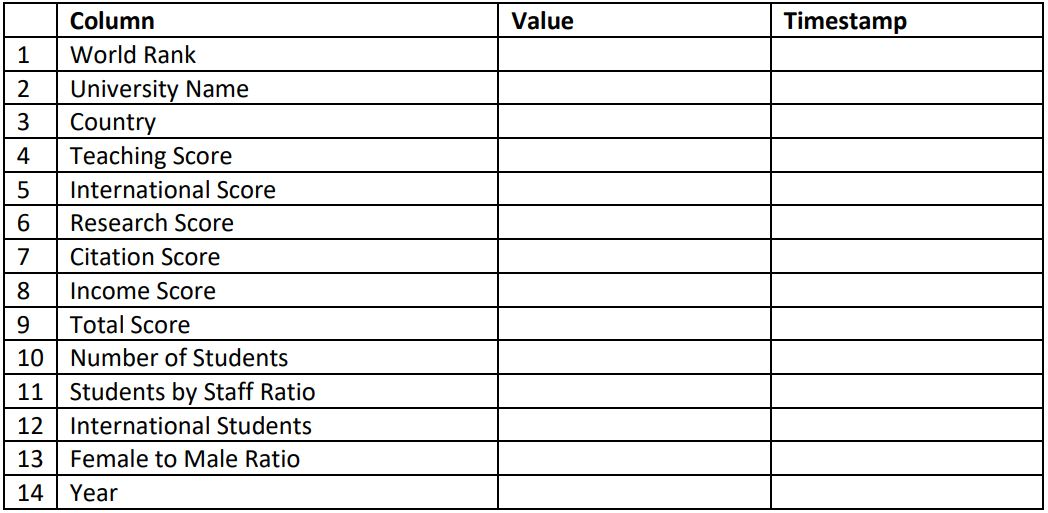
\includegraphics[width=\textwidth]{images/milepael4/rawObject.JPG}
\end{figure}

\textbf{Pseudo-Kode}
\begin{enumerate}
  \item Register each field from user input
  \item Save data as an object
  \item Post object to database
\end{enumerate}

% Aggregering 2 %
\textbf{Top 10 Universities By Diversity}\\
I dette dataobjektet rangeres hvert universitet ut ifra en ny faktor som vi har skapet kalt "Diversity Score". Dette er en sammenslåing av følgende felt fra Rådata-objektet: Number of Students, International Students, Female To Male. På denne måten kan man få en oversikt over hvilke skoler som har mest mangfoldig studentmiljø. Til slutt skal dette ha en limit på 10.

Vi endte opp med å ikke bruke dette dataobjektet, fordi det var mer utfordrende enn vi trodde å regne ut diversity.

\FigureCounter
\begin{figure}[H]
  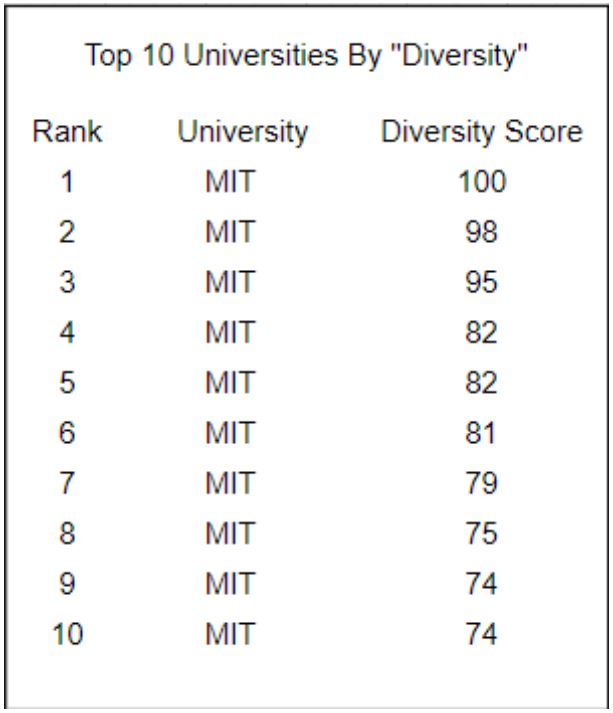
\includegraphics[scale=0.5]{images/milepael4/topTenUnis.JPG}
\end{figure}

\textbf{Pseudo-Kode}
\begin{enumerate}
  \item Calculate diversity factor
  \item Group By University
  \item Limit by 10
\end{enumerate}

\pagebreak
% Aggregering 3 %
\textbf{Average Score Per Year}\\
Denne aggregeringen visualiserer gjennomsnittet av den sammenlagte poengsummen fra alle skoler per år. Dette kan være interessant for å se hvilke år som gikk generelt gikk bedre eller verre for studenter rundt om i verden.

\FigureCounter
\begin{figure}[H]
  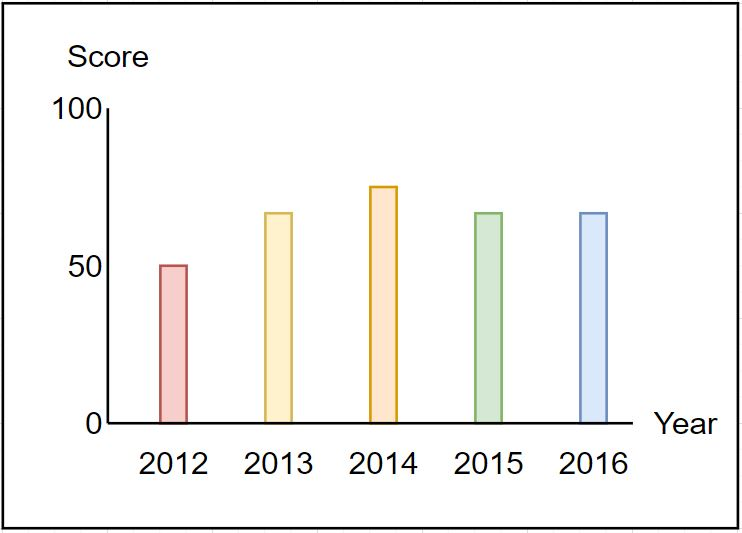
\includegraphics[scale=0.5]{images/milepael4/averageScorePerYear.JPG}
\end{figure}

\textbf{Pseudo-Kode}
\begin{enumerate}
  \item Calculate average total score
  \item Define number of students interval
  \item Group by number of students interval
\end{enumerate}

\pagebreak
% Aggregering 4 %
\textbf{Top 10 universities by female ratio}\\
Denne aggregeringen viser top ti universiteter med flest kvinnelig fordeling i studentene sine i året 2016. Den skal vise fram navnet på universitetet, hvilket land det ligger i, og fordelingen mellom menn og kvinner, hvor fordelingen vil bli vist i antall prosent.

\textbf{Pseudo-Kode}
\begin{enumerate}
  \item Hente country, university name og female male ratio
  \item Splitte female male ratio på kolon og hente ut female ratio
  \item Filtrer på året 2016
\end{enumerate}

\pagebreak
% Aggregering 5 %
\textbf{Top 10 universities by male ratio}\\
Denne aggregeringen er tilsvarende \textit{Top 10 universities by female ratio}, bortsett fra at man ser på den mannlige fordelingen.

\textbf{Pseudo-Kode}
\begin{enumerate}
  \item Hente country, university name og female male ratio
  \item Splitte female male ratio på kolon og hente ut male ratio
  \item Filtrer på året 2016
\end{enumerate}

\pagebreak
\subsubsection{Opprettelse av databasen}
Det første må gjøre er å opprette et "keyspace" i Cassandra. Dette tilsvarer en database i MySQL. Her opprettes keyspacet "university" hvor alle kommende tables havner i. Det er viktig å merke seg \lstinline{WITH replication}, siden den bestemmer hvordan datakopier spres utover en klynge. For denne løsning brukes \textit{SimpleStrategy} med \textit{replication factor} av 1.

\txt{code/milepael4/createNamespace.txt}

Replikasjonsstrategien bestemmer hvordan datakopiene distribueres rundt om i \textit{Cassandra ringen}, der en ring representerer en klynge av noder, også kalt et datasenter. Som en tommelfingelregel brukes SimpleStrategy når man bare har et datasenter, ellers brukes \textit{NetworkTopologyStrategy}. Begge strategiene populerer datasettene node for node med klokken, forskjellen er at SimpleStrategy kun populerer et datasett, mens NetworkTopologyStrategy populererer flere.

\FigureCounter
\begin{figure}[H]
  \centering
  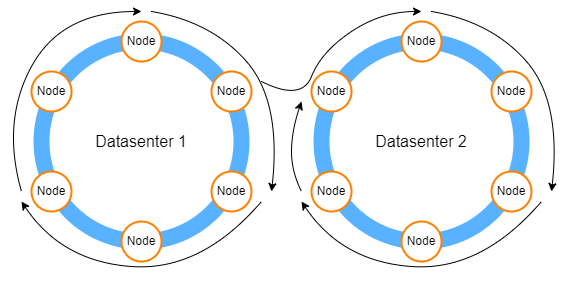
\includegraphics[scale=0.5]{images/milepael6/replicationstrategy.drawio.png}
  \caption{Figuren viser hvordan de to replikasjonsstrategiene distribuerer datakopier utover klyngene. SimpleStrategy vil kun distribuere til datasenter 1, mens NetworkTopologyStrategy vil starte i datasenter 1 og jobbe seg utover datasenter 2.}
\end{figure}

Videre bestemmer replikasjonsfaktoren hvor mange datakopier som skal spres utover klyngen, for eksempel i en klynge med seks noder og replikasjonsfaktor på tre, vil halvparten av nodene være tilgitt en datakopi. På denne måten forsørger man at data er utilgjengelig dersom en node skulle feile. Legg merke til at det ikke er lov til å ha en replikasjonsfaktor større enn antall noder i en klynge. 

I Cassandra tar man også hensyn til noe kalt for \textit{Cassandra consistensy level}, som er minimum antall noder som må annerkjenne lese- og skrive-spørringer før det kan kalles en gyldig operasjon. Dette er en verdi som kan settes selv. Som regel brukes Cassandra verdien \textit{Local Quorum}, som defineres slik: \lstinline{LOCAL_QUORUM = (replication_factor/2) + 1}, denne rundes ned til nærmeste heltall.

Det neste er å opprette selve tabellene i Cassandra via \lstinline{CREATE TABLE} setningen. Her er det viktig å passe på at både kolonnenavn og datatyper stemmer med datasettet, ellers kan man ikke sende dataen videre til Cassandra. I tillegg krever Cassandra minst én \textit{primærnøkkel}, noe som var problamtisk da det opprinnelige datasettet ikke hadde noen id. Man kunne løst dette på flere måter, men jeg valgte å manuelt legge til dette i LibreOffice. Ellers kan man bruke følgende kommando i spark-shell: \lstinline{myDf.withColumn("id", monotonically_increasing_id)}.

\txt{code/milepael4/createTable.txt}

\subsubsection{Hente ut data}
\txt{code/milepael4/getDataColumnDB.txt}

\subsubsection{Sette inn data}
\txt{code/milepael4/insertDataColumnDB.txt}

\subsubsection{Hvordan eksisterende data oppdateres}
\begin{itemize}
  \item Ny data kommer inn
  \item Data/kommando verifisering
  \item Sjekker om raden er ledig
  \item Ledig - oppdaterer raden
  \item Ikke ledig - lager ny rad for samme data
  \item Data oppdateres på aktuelle noder
\end{itemize}